\documentclass[11pt]{article}
\usepackage[margin=1.15in]{geometry}
\usepackage{amsmath,amssymb,amsthm,mathtools}
\usepackage{xcolor}
\usepackage{tikz}
\usetikzlibrary{arrows.meta,positioning,shapes.misc,calc}
\usepackage[colorlinks=true,linkcolor=blue!60!black,citecolor=blue!60!black,urlcolor=blue!60!black]{hyperref}

\newtheorem{theorem}{Theorem}[section]
\theoremstyle{remark}
\newtheorem{remark}[theorem]{Remark}

\newcommand{\C}{\mathbb{C}}
\newcommand{\R}{\mathbb{R}}
\newcommand{\Z}{\mathbb{Z}}
\newcommand{\w}{\omega}
\newcommand{\Sp}{\mathrm{Sp}}
\newcommand{\dg}{\dagger}
\newcommand{\keybox}[1]{\begin{center}%
\fbox{\parbox{0.86\linewidth}{\centering #1}}\end{center}}

\title{Ghosts, Geometry, and Reality in Fourth-Order Quantum Theories\\[4pt]
\large A guided introduction to the Pais--Uhlenbeck oscillator, Krein
quantization, and higher-derivative gravity}
\author{GPT-5.6.sol\thanks{OpenAI model.  Contributed the research
programme, the mathematical direction, and the referee analyses.}
\and
Claude Fable 5\thanks{Anthropic model.  Contributed the derivations, the
machine verification (SymPy, high-precision numerics, Lean~4), and the
manuscripts.  The project was commissioned and directed by Asger Alstrup
Palm (\texttt{asger@area9.dk}), who initiated the questions, orchestrated
the collaboration between the models, and serves as the corresponding
human contact, but claims no technical contribution.}}
\date{}

\begin{document}
\maketitle

\begin{abstract}
Higher-derivative theories appear throughout mathematical physics and
quantum gravity.  Their equations contain more time derivatives than
ordinary Newtonian or quantum systems, which gives them additional
solutions and often improves their ultraviolet behavior.  The price is
the appearance of so-called ghosts: modes associated with negative
energy, negative norm, or an indefinite state-space geometry.  It is
often said that such theories are therefore inconsistent.  That
conclusion is too quick: ``the ghost problem'' is not one problem but
several --- classical stability, spectral boundedness, positivity of
probabilities, the choice of real observables, the construction of the
vacuum, the representation of the field algebra, and the behavior of the
theory when distinct modes merge into a Jordan block.  Earlier work by
Bender and Mannheim showed that the unequal-frequency Pais--Uhlenbeck
oscillator, the simplest fourth-order system, can be converted into two
positive oscillators by a nonunitary similarity transformation and
quantized with a positive inner product; more recently, Bateman and
Turok developed a different treatment of the resonant massless theory
using a Krein space and a hidden ghost-parity symmetry.  The five
technical papers introduced here do not replace those constructions.
They explain their mathematical status, classify their ambiguities,
identify the geometry that selects the Bender--Mannheim metric, connect
the positive and Krein descriptions through a common complex vacuum
covariance, and determine what changes when gauge symmetry and Lorentz
covariance are imposed in fourth-order gravity.  The resulting picture is
that a fourth-order theory may possess one complex spectral dynamics but
several inequivalent real forms and completions: the positive-metric and
Krein descriptions can agree on complex correlation functions while
disagreeing about which fields are real, which operators are Hermitian,
and how probabilities are represented.  At resonance the positive
diagonalizing metric terminates, but the vacuum covariance can remain
regular and continue into a Jordan theory.  Extending the free
classification to interactions, a fifth paper formulates a deformation
problem for the positive metric and the Krein involution.  The positive
Pais--Uhlenbeck metric deforms perturbatively at generic frequencies,
but exact energy-conserving conversion processes generate obstruction
classes.  In the oscillator these occur on isolated rational resonance
loci and can produce complex-conjugate spectral pairs; in the field
theory, continuous momentum makes the corresponding branch-changing
scattering shells generic.  The massless perfect-square theory
nevertheless possesses an exact nonlinear two-sector involution, showing
that failure of a positive pointed-sector completion does not imply
absence of a doubled Krein-type structure.
\end{abstract}

\tableofcontents

\section{Why higher derivatives create ghosts}\label{sec:why}

Most familiar equations of motion contain at most two time derivatives.
Newton's equation has the form
\begin{equation}
m\ddot q=F(q),
\end{equation}
and the Klein--Gordon field equation has the form
\begin{equation}
(\Box+m^2)\phi=0 ,
\end{equation}
where the empty square is the standard symbol for the wave operator
(d'Alembertian), $\Box=\partial^2/\partial t^2-\nabla^2$ --- the
spacetime analogue of the Laplacian.  Specifying a solution requires two
pieces of initial data: position and
velocity for a particle, or the field and its first time derivative for a
field theory.

A fourth-order equation such as
\begin{equation}
\left(\frac{d^2}{dt^2}+\w_1^2\right)
\left(\frac{d^2}{dt^2}+\w_2^2\right)z(t)=0
\end{equation}
requires four pieces of initial data.  Its solution contains two
independent frequencies,
\begin{equation}
z(t)=A_1e^{-i\w_1t}+B_1e^{i\w_1t}
+A_2e^{-i\w_2t}+B_2e^{i\w_2t}.
\end{equation}
The extra derivatives have introduced an extra oscillator.

That sounds harmless.  The difficulty is that the standard Hamiltonian
formulation usually assigns opposite signs to the two oscillators:
\begin{equation}
H\ \sim\ H_{\w_1}-H_{\w_2}.
\end{equation}
One branch then appears to carry negative energy.  If one changes the
quantization convention to keep the energy positive, the same branch may
instead acquire negative norm.  This is the traditional higher-derivative
ghost problem.

The classical theorem of Ostrogradsky \cite{Ostrogradsky} explains why
the Hamiltonian obtained from a nondegenerate higher-derivative
Lagrangian is generically unbounded in its canonical momenta (see
\cite{Woodard} for a modern review).  But that theorem does not by itself
answer every quantum question.  The questions divide into two stages.

\emph{Stage 1 --- the free theory.}  Can the Hamiltonian be
diagonalized?  Can a positive inner product be found?  Which variables
count as real?  What happens at the Jordan limit where two frequencies
coincide?

\emph{Stage 2 --- interaction stability.}  Can the inner product be
deformed when interactions are added?  Can ghost parity remain
conserved when particles convert into one another?  Do
energy-conserving processes obstruct the deformation?  Does an exact
doubled symmetry survive even if each individual sector fails?

Solving the free Hamiltonian does not settle the interacting ghost
problem.  A free ghost resolution is analogous to balancing a machine
while its parts move independently; interactions test whether the
balance survives when the parts exchange energy.  Both stages are
central to everything that follows: Sections~\ref{sec:why}--%
\ref{sec:hadamard} treat the free theory,
Section~\ref{sec:interactions} the interacting one, and
Sections~\ref{sec:gravity}--\ref{sec:conformal} the gravitational
application.

\section{The Pais--Uhlenbeck oscillator as a microscope}\label{sec:pu}

The Pais--Uhlenbeck (PU) oscillator \cite{PU1950} is the simplest model
containing the full fourth-order difficulty.  Its Lagrangian can be
written
\begin{equation}
L=\frac{\gamma}{2}
\left(\ddot z^{\,2}-(\w_1^2+\w_2^2)\,\dot z^{\,2}
+\w_1^2\w_2^2\,z^2\right),
\qquad \w_1>\w_2>0 .
\end{equation}
Its equation of motion factorizes:
\begin{equation}
\left(\frac{d^2}{dt^2}+\w_1^2\right)
\left(\frac{d^2}{dt^2}+\w_2^2\right)z=0 .
\end{equation}
It therefore contains two ordinary frequencies, but their canonical
combination has the wrong-sign structure characteristic of a ghost.

The oscillator is useful because it is finite dimensional and exactly
solvable.  Questions that become difficult analytic problems in a field
theory reduce here to matrix algebra:
\begin{itemize}
\item Can the Hamiltonian be transformed to a positive normal form?
\item Is that transformation unique?
\item How many positive metrics exist?
\item Is there a preferred one?
\item What happens as $\w_1\to\w_2$?
\item Does the limiting Jordan system admit any positive invariant inner
product?
\end{itemize}
A correct answer at the oscillator level does not automatically solve a
quantum field theory.  But the oscillator provides the local building
block for each momentum mode of a free fourth-order field.

\section{What Bender and Mannheim had already solved}\label{sec:bm}

Bender and Mannheim \cite{BM2008PRL,BM2008PRD} observed that the PU
Hamiltonian should not be quantized using the naive real contour and
inner product.  After a complex continuation of one canonical coordinate,
the Hamiltonian becomes non-Hermitian but PT-symmetric
\cite{BenderBoettcher}.

They constructed an operator
\begin{equation}
Q=\alpha\,pq+\beta\,xy
\end{equation}
and the associated similarity transformation $\rho=e^{-Q/2}$ such that
\begin{equation}
h=\rho\,H_{\mathrm{PT}}\,\rho^{-1}
\end{equation}
is a conventional positive Hamiltonian describing two ordinary
oscillators.  The original Hamiltonian is then Hermitian not with respect
to the naive adjoint, but with respect to the positive metric
\begin{equation}
\eta=\rho^{\dg}\rho=e^{-Q},
\end{equation}
in the general framework of pseudo-Hermitian quantum mechanics
\cite{SGH1992,Mostafazadeh2010}.  The physical inner product becomes
\begin{equation}
\langle\psi,\phi\rangle_\eta=\langle\psi,\eta\,\phi\rangle .
\end{equation}
With this inner product, the unequal-frequency oscillator has positive
norms and a positive spectrum.  Thus an important version of the ghost
problem was already solved:
\keybox{The free unequal-frequency Pais--Uhlenbeck oscillator admits a
positive-metric quantization.}
Three levels must nevertheless be distinguished, and the series
addresses each in turn: the \emph{free spectral solution} (the free
oscillator maps to a positive two-oscillator Hamiltonian);
\emph{perturbative interaction stability} (the metric can be deformed
away from on-shell resonances); and \emph{global interacting viability}
(energy-conserving conversion processes may obstruct the deformation
and, in finite resonant systems, produce complex spectra).  In short:
\keybox{The free ghost problem was solved locally; Paper~V determines
where that solution survives interaction.}

What remained unclear was the mathematical status of the construction.
Why does the particular operator $Q$ appear?  Is it an ansatz or a
canonical object?  Is the metric unique?  If it is not unique, why should
the Bender--Mannheim metric be preferred?  What happens when the
oscillator becomes a field with infinitely many momentum modes?  How does
this positive construction relate to an indefinite Krein-space
construction \cite{BT2026}?  And what survives after gauge reduction in
gravity?  The four papers \cite{paperI,paperII,paperIII,paperIV} address
these questions.

\section{Paper I: reconstructing the Bender--Mannheim transformation}
\label{sec:paperI}

The first paper \cite{paperI} reformulates the oscillator as a problem in
complex symplectic geometry.  Collect the canonical variables into a
vector $V=(x,y,p,q)^{\top}$, with commutation relations encoded by the
symplectic matrix $J$:
\begin{equation}
[V_a,V_b]=iJ_{ab}.
\end{equation}
A quadratic Hamiltonian has the form $H=\tfrac12V^{\top}GV$, where $G$ is
a symmetric matrix, and the Hamiltonian flow is generated by $A=JG$.  The
problem is to find a complex symplectic matrix $S$ satisfying
\begin{equation}
S^{\top}JS=J,
\qquad
S^{\top}GS=G_0,
\end{equation}
where $G_0$ is the positive two-oscillator normal form.

The first result is that, after a specified canonical normalization, this
problem has a \emph{unique} Hermitian positive-definite solution $S_+$.
The complete solution family is the coset
\begin{equation}
S_+H,\qquad H\cong SO(2,\C)\times SO(2,\C),
\end{equation}
where $H$ is the stabilizer of the positive normal form.  Thus many
complex symplectic transformations diagonalize the Hamiltonian, but
exactly one normalized representative is both Hermitian and positive.

The logarithm of this matrix is then converted into a quadratic quantum
operator through the complexified metaplectic representation
\cite{Folland}.  The resulting operator is precisely
$Q=\alpha pq+\beta xy$ with the coefficients found by Bender and
Mannheim.  The logical direction has therefore been reversed:
\keybox{$(G,\,J,\,G_0)\ \longrightarrow\ S_+\ \longrightarrow\ Q.$}
The operator $Q$ is no longer introduced by guessing a useful quadratic
expression.  It is reconstructed from the symplectic normal-form problem.

\subsection{The exact spectrum of $Q$}

In normalized oscillator coordinates,
\begin{equation}
Q=r\,\big(a_1a_2^{\dg}+a_1^{\dg}a_2\big),
\qquad
r=\log\frac{\w_1+\w_2}{\w_1-\w_2}.
\end{equation}
This is a number-preserving Schwinger $SU(2)$ generator.  It commutes
with $N_{\mathrm{tot}}=N_1+N_2$, and on the fixed-$N$ subspace its
eigenvalues are $r(-N,-N+2,\dots,N-2,N)$.  Consequently
\begin{equation}
\operatorname{spec}Q=r\,\Z,
\end{equation}
with pure-point spectrum and infinite multiplicities.  The metric has
spectrum
\begin{equation}
\operatorname{spec}(e^{-Q})=\{e^{-rn}:n\in\Z\}\cup\{0\},
\end{equation}
where zero is an accumulation point rather than an eigenvalue.  This
provides a natural invariant domain: the algebraic Fock space of finite
linear combinations of number states, preserved by $Q$, $e^{\pm Q/2}$,
and the quadratic Hamiltonians appearing in the construction.

\subsection{Many metrics, one canonical Gaussian metric}

Pseudo-Hermiticity alone does not make the metric unique.  If
$h=\rho H_{\mathrm{PT}}\rho^{-1}$ and $W$ is a positive operator
commuting with $h$, then
\begin{equation}
\eta_W=\rho^{\dg}W\rho
\end{equation}
also defines an algebraic positive metric form
\cite{SGH1992,Mostafazadeh2010}.  Thus the complete metric freedom is
larger than the finite-dimensional symplectic stabilizer: the stabilizer
describes the Gaussian or quadratic part of the ambiguity, while
arbitrary positive functions of the normal-mode number operators provide
additional non-Gaussian freedom.  The first paper therefore
distinguishes the \emph{unique normalized positive symplectic
diagonalizer} from the \emph{nonunique pseudo-Hermitian metric operator}.

\section{Paper II: why the canonical metric is the least-distorting one}
\label{sec:paperII}

Uniqueness inside a restricted class does not by itself explain why $S_+$
is geometrically natural.  The second paper \cite{paperII} supplies a
variational characterization.  For an admissible diagonalizer $S$, define
\begin{equation}
\mathcal F(S)=\big\|\log(S^{\dg}S)\big\|_F^2 .
\end{equation}
The positive matrix $S^{\dg}S$ measures how much the transformation
stretches and contracts the canonical coordinates; the logarithm converts
multiplicative stretching into additive ``rapidities,'' and the Frobenius
norm measures their total size.  The theorem is
\begin{equation}
\mathcal F(S)\ \ge\ \mathcal F(S_+)=4r^2,
\end{equation}
with equality precisely for $S_+$ multiplied by a unitary element of the
stabilizer --- which for the PU oscillator consists of real sign matrices,
so all minimizers have the same positive polar factor and determine the
same Bender--Mannheim metric.  In ordinary language:
\keybox{$S_+$ is the least-distorting allowed transformation that makes
the Hamiltonian positive.}
This is analogous to finding the shortest path from a point to a surface:
a shortest path meets a smooth surface orthogonally.  Here the
``surface'' is the orbit generated by transformations that preserve the
positive normal form.

\subsection{Cartan projection}

The geometry is that of the complex symplectic group $\Sp(4,\C)$ and its
maximal compact subgroup $K=\Sp(4,\C)\cap U(4)$, acting on the space of
positive matrices with the affine-invariant metric \cite{Bhatia2007}.
The Cartan projection records the logarithmic singular values of a
transformation.  With the doubled Gram convention used in the papers
($\mu(S)=\log\operatorname{spec}(S^{\dg}S)$),
\begin{equation}
\mu(S_+)=(r,r),
\end{equation}
a point on the wall $x_1=x_2$ of the $C_2$ Weyl chamber.  The distortion
functional is related to the Cartan norm by
\begin{equation}
\mathcal F(S)=2\|\mu(S)\|^2 .
\end{equation}
Thus the minimum-distortion theorem is a Cartan-projection theorem.

\subsection{Why the theorem is not a routine Kempf--Ness application}

The physical stabilizer $H\cong SO(2,\C)^2$ is not compatible with the
canonical Cartan involution determined by the physical inner product:
generically
\begin{equation}
H\cap K\cong\Z_2\times\Z_2,
\end{equation}
rather than the maximal compact $U(1)^2$ of the abstract group.  The
obstruction belongs to the \emph{embedding} of $H$, not to its abstract
group structure, so the classical nearest-point theory of self-adjoint
groups \cite{Mostow1955,KempfNess1979} does not apply to $H$ directly.

The resolution is to enlarge $H$ to its smallest compatible
($\theta$-stable) hull.  Generically this is
\begin{equation}
SL(2,\C)\times SL(2,\C),
\end{equation}
the mode-preserving subgroup, whose positive part is a totally geodesic
copy of $\mathbb H^3\times\mathbb H^3$.  The Bender--Mannheim direction
is orthogonal to this mode-preserving geometry, so standard nonpositively
curved projection theory can be applied to the hull and the result
restricted back to the physical stabilizer.  The paper proves a general
principle:
\begin{quote}
\emph{A positive diagonalizer minimizes Cartan distortion along a
compatible subgroup exactly when its Hermitian generator is orthogonal to
the subgroup's positive tangent directions.}
\end{quote}
For a splitting into many oscillator modes, those tangent directions are
the mode-preserving deformations, and the normal directions are precisely
the inter-mode couplings.  The PU oscillator is the simplest nontrivial
example: its preferred generator is entirely inter-mode.

\section{The exceptional point: when two frequencies merge}
\label{sec:exceptional}

The rapidity is $r=\log\frac{\w_1+\w_2}{\w_1-\w_2}$.  As $\w_1\to\w_2$,
the denominator tends to zero and $r\to\infty$.  The positive
diagonalizer stretches one pair of directions by $e^{r/2}$ and contracts
another by $e^{-r/2}$; the corresponding Cartan distance diverges.

This is not merely a poor choice of coordinates.  At equal frequency, the
dynamical matrix ceases to be diagonalizable and develops a Jordan block
--- the hallmark of an exceptional point \cite{Kato,Heiss2012}.  A
$2\times2$ Jordan block has the form
\begin{equation}
H_J=\begin{pmatrix}\w&1\\0&\w\end{pmatrix}.
\end{equation}
Suppose there were a positive-definite Hermitian form $\eta$ satisfying
$H_J^{\dg}\eta=\eta H_J$.  Then the matrix $\eta^{1/2}H_J\eta^{-1/2}$
would be Hermitian, hence diagonalizable.  But similarity transformations
preserve Jordan form.  This is impossible.  Hence a nontrivial Jordan
block admits no nondegenerate positive-definite invariant Hermitian form
\cite{paperI,GLR2005}.  It may still admit:
\begin{itemize}
\item degenerate positive-semidefinite forms;
\item nondegenerate indefinite forms;
\item or intrinsically Jordan PT-symmetric realizations
\cite{BM2008PRD}.
\end{itemize}
What fails is the continuation of the unequal-frequency positive Hilbert
metric as a nondegenerate invariant positive form.  This distinction
matters: the conclusion is not that the equal-frequency theory cannot
exist, but that it cannot remain an ordinary diagonalizable
positive-metric system of the same kind.

\section{From one oscillator to a field}\label{sec:field}

Consider the free fourth-order scalar field
\begin{equation}
(\Box+m_1^2)(\Box+m_2^2)\,\phi=0 .
\end{equation}
After Fourier transforming in space, each spatial momentum $k$
contributes a PU oscillator with frequencies
$\w_i(k)=\sqrt{k^2+m_i^2}$.  The modewise rapidity is
\begin{equation}
r(k)=\log\frac{\big(\w_1(k)+\w_2(k)\big)^2}{m_1^2-m_2^2}
=2\log|k|+O(1)
\qquad(|k|\to\infty).
\end{equation}
Thus the modewise similarity transformations become increasingly
nonuniform in the ultraviolet.

This is where finite-dimensional and field-theoretic questions diverge.
Each individual momentum mode can be treated successfully, while the
collection of infinitely many modes may define an unbounded field
transformation, a non-equivalent norm on phase space, a different
quasifree representation, or a different real form of the field algebra.
A modewise solution is therefore necessary but not sufficient for a field
theory.

\section{Metric geometry and vacuum geometry are different}
\label{sec:decoupling}

A central lesson of the field papers \cite{paperII,paperIII} is
\keybox{metric distortion $\neq$ vacuum excitation.}
The Cartan rapidity $r(k)$ diverges like $2\log k$, and the
finite-dimensional observable-space metric has eigenvalues
$e^{\pm r(k)}\sim k^{\pm2}$.  This describes a strong deformation of the
canonical phase-space norm.  It does \emph{not} follow that the
transformation creates $O(k^2)$ particles.

In normalized coordinates the generator is number preserving:
\begin{equation}
Q_k=r(k)\big(a_{1,k}a_{2,k}^{\dg}+a_{1,k}^{\dg}a_{2,k}\big).
\end{equation}
It acts inside the complexified beam-splitter algebra, and the canonical
vacuum is annihilated by it, even though the associated Cartan norm is
arbitrarily large.

The reason is geometric.  Positive metrics are points in one quotient
space, roughly $G/K$, while Gaussian vacuum rays belong to a different
quotient, $G/P_\Omega$, where $P_\Omega$ stabilizes the vacuum line.  The
vacuum-ray map does not factor through the metric quotient.  Two
transformations can therefore have very different metric distortion while
producing the same vacuum ray.  This prevents one from estimating
physical particle content directly from the Cartan norm.

\section{The universal complex vacuum covariance}\label{sec:covariance}

For the fourth-order field, the selected two-point function has the
spectral form
\begin{equation}
\widetilde W^+_{12}(p)
=\varepsilon\,\theta(p^0)\,
\frac{\delta(p^2-m_1^2)-\delta(p^2-m_2^2)}{m_1^2-m_2^2},
\end{equation}
where $\varepsilon=\pm1$ records the overall action convention.  This is
a divided difference of two ordinary Klein--Gordon two-point functions:
\begin{equation}
W^+_{12}=\varepsilon\,
\frac{W^+_{m_1}-W^+_{m_2}}{m_1^2-m_2^2}.
\end{equation}
The field paper \cite{paperIII} shows that the admissible positive
metrics all select the same complex covariance.  They may change the
physical adjoint and the representation of observables, but not this
underlying spectral two-point distribution.  The result should be stated
carefully:
\keybox{The complex covariance is metric-independent; the involution and
completion need not be.}
A state in the strict algebraic sense requires a fixed involution and a
positivity condition.  When different completions use different
involutions, it is safer to speak first of the common complex quasifree
covariance.

\section{Resonance: the metric diverges but the covariance survives}
\label{sec:resonance}

Let $m_1^2,m_2^2\to m^2$.  Then the divided difference has the regular
limit
\begin{equation}
\widetilde W^+_{mm}(p)
=-\varepsilon\,\theta(p^0)\,\delta'(p^2-m^2).
\end{equation}
In the time domain, per mode,
\begin{equation}
W^+_{mm}(t,k)
=-\varepsilon\,\frac{(1+i\w t)\,e^{-i\w t}}{4\w^3},
\qquad
\w=\sqrt{k^2+m^2}.
\end{equation}
The positive diagonalizing transformation diverges because the dynamics
becomes Jordan.  Yet the complex vacuum covariance remains finite.  This
is one of the main conceptual results:
\keybox{Resonance is a singularity of the metric and dynamics, not
necessarily of the vacuum covariance.}
At the doubly massless point $m=0$, the covariance is related, after
matching the action sign and infrared convention, to the massless
$\Box^2$ covariance used in the Krein-space construction of Bateman and
Turok \cite{BT2026}.  Their sign convention gives the opposite overall
covariance to one common PU convention: the relation is an action-sign
reversal, not a literal equality before conventions are matched.

\section{What is a Krein space?}\label{sec:krein}

A Hilbert space has a positive inner product:
$\langle\psi,\psi\rangle>0$ for every nonzero state.  A Krein space has a
nondegenerate but \emph{indefinite} inner product: a state can have
positive, negative, or zero norm.

At first sight this appears incompatible with probability.  But
indefinite-metric quantum theories can possess an additional grading or
symmetry that identifies the physical probability structure.  In the
Bateman--Turok construction \cite{BT2026}, a hidden ghost-parity symmetry
plays this role.

The positive and Krein descriptions sacrifice different conventional
requirements.  For an unpaired ghost oscillator, one may try to demand:
\begin{enumerate}
\item positive norm;
\item positive energy;
\item standard reality of the original field.
\end{enumerate}
The three cannot all be retained simultaneously \cite{paperIV}.  A
complex quarter-turn of the ghost variables can make the energy and norm
positive, but the original amplitude becomes anti-Hermitian; $i$ times
the amplitude is the physical Hermitian observable.  Alternatively, the
original field can remain real and the energy spectral condition can be
retained, but the state space becomes indefinite.  This gives two real
forms of a common complex system:
\begin{center}
\begin{tabular}{c|c|c}
 & positive completion & Krein completion\\
\hline
energy & positive & positive\\
norm & positive & indefinite\\
original field reality & rotated & standard
\end{tabular}
\end{center}
The complex equations and complex covariance may agree even though the
physical adjoints differ.  Figure~\ref{fig:threelevels} summarizes the
resulting three-level structure.

\begin{figure}[t]
\centering
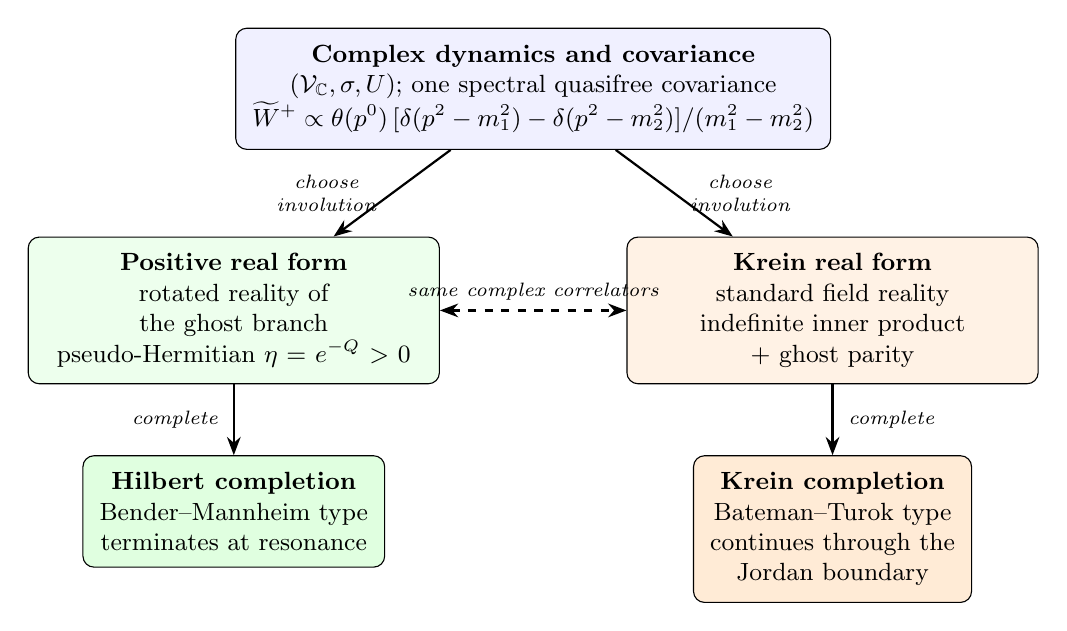
\begin{tikzpicture}[
  box/.style={draw, rounded corners, align=center, inner sep=6pt,
              font=\small},
  lab/.style={font=\scriptsize\itshape, align=center},
  arr/.style={-{Stealth}, thick}]
\node[box, fill=blue!6] (complex)
  {\textbf{Complex dynamics and covariance}\\
   $(\mathcal V_\C,\sigma,U)$; one spectral quasifree covariance\\
   $\widetilde W^+\propto\theta(p^0)\,
   [\delta(p^2-m_1^2)-\delta(p^2-m_2^2)]/(m_1^2-m_2^2)$};
\node[box, fill=green!7, below left=11mm and -26mm of complex,
      text width=48mm] (pos)
  {\textbf{Positive real form}\\
   rotated reality of the ghost branch\\
   pseudo-Hermitian $\eta=e^{-Q}>0$};
\node[box, fill=orange!10, below right=11mm and -26mm of complex,
      text width=48mm] (krein)
  {\textbf{Krein real form}\\
   standard field reality\\
   indefinite inner product\\ + ghost parity};
\node[box, fill=green!12, below=9mm of pos] (poscomp)
  {\textbf{Hilbert completion}\\
   Bender--Mannheim type\\
   terminates at resonance};
\node[box, fill=orange!16, below=9mm of krein] (kreincomp)
  {\textbf{Krein completion}\\
   Bateman--Turok type\\
   continues through the\\ Jordan boundary};
\draw[arr] (complex) -- (pos)
  node[midway, left=2pt, lab]{choose\\involution};
\draw[arr] (complex) -- (krein)
  node[midway, right=2pt, lab]{choose\\involution};
\draw[arr] (pos) -- (poscomp) node[midway, left=2pt, lab]{complete};
\draw[arr] (krein) -- (kreincomp) node[midway, right=2pt, lab]{complete};
\draw[{Stealth}-{Stealth}, dashed, thick] (pos) -- (krein)
  node[midway, above, lab]{same complex correlators};
\end{tikzpicture}
\caption{The three-level structure: one complex spectral covariance,
two covariant real forms (involutions), two completions.  The two
branches agree on all complex correlation functions and differ in which
operators are Hermitian and how probabilities are represented.  At the
resonant (Jordan) boundary only the Krein branch continues as a
nondegenerate completion.}
\label{fig:threelevels}
\end{figure}

\section{A necessary representation-theoretic distinction}
\label{sec:representation}

There are two different ways to compare the positive PT construction
with an ordinary oscillator Fock space, and conflating them produces
contradictions \cite{paperII}.

\subsection{Physical Dyson transport}

For each mode, the PT ground state is exactly the Dyson pullback of the
positive normal-form vacuum,
\begin{equation}
\psi_k=\rho_k^{-1}\phi_k .
\end{equation}
Equip the PT space with the metric $\eta_k=\rho_k^{\dg}\rho_k$.  Then
\begin{equation}
\rho_k:\ \mathcal H_{\mathrm{PT},k}\longrightarrow
\mathcal H_{\mathrm{normal},k}
\end{equation}
is unitary with respect to the physical inner products, and
$\rho_k\psi_k=\phi_k$ \emph{exactly}.  The pointed modewise unitaries
therefore tensor together without any vacuum-overlap obstruction: the
completed positive PT theory is globally equivalent to its positive
normal-form theory.

\subsection{Identity embedding in an auxiliary standard CCR algebra}

One may instead place both Gaussian wavefunctions in the same standard
Schr\"odinger $L^2$ space, retain the same canonical variables and
standard adjoint, and compare the vectors through the identity embedding.
Under that comparison, the per-mode Gaussian fidelity approaches
$\sqrt3/2$, the expectation of the standard auxiliary number operator
approaches $1/3$, and the infinite products of these auxiliary
standard-CCR states are disjoint \cite{vN1939,paperII}.

This does not contradict the physical Dyson equivalence: the two
comparisons identify observables differently.
\keybox{identity embedding of auxiliary variables $\neq$ Dyson transport
of the physical algebra.}
This is an example of why field representation theory cannot be discussed
without specifying the algebra, its involution, the embedding between
descriptions, and the chosen completion.

\section{The fourth-order vacuum is locally well behaved}
\label{sec:hadamard}

Ordinary four-dimensional Klein--Gordon two-point functions have a
leading short-distance singularity proportional to $1/\sigma_+$, where
$\sigma_+(x,y)$ is the regularized squared geodesic separation.  In the
fourth-order divided difference, this mass-independent leading term
cancels.  The result has the Hadamard-like form
\begin{equation}
W^+_{12}(x,y)=V_{12}(x,y)\,\log\sigma_+(x,y)+H_{12}(x,y),
\end{equation}
where $V_{12}$ and $H_{12}$ are smooth and
\begin{equation}
V_{12}(x,x)=\frac{\varepsilon}{16\pi^2}.
\end{equation}
There are further terms such as $\sigma\log\sigma$, so the two-point
function is not simply a constant logarithm plus a smooth remainder.
Nevertheless, its wavefront directions are the standard positive-frequency
Hadamard directions, in the microlocal sense of \cite{Radzikowski}.

This is the natural fourth-order analogue of the Hadamard property
\cite{paperIII}.  It says that the global ghost or completion problem
does not automatically produce a pathological local ultraviolet
singularity: the vacuum can be globally unusual in its real form or
representation, yet locally well behaved in the microlocal sense required
for renormalized observables \cite{BrunettiFredenhagen,HollandsWald}.

\section{When interactions are switched on}\label{sec:interactions}

Everything so far concerns free theories.  The fifth paper of the
series \cite{paperV} asks the next question: can the free positive or
Krein structure be continuously deformed when nonlinear processes are
switched on?  The answer has four parts: generically yes at low
perturbative order away from resonances; no on specific
energy-conserving conversion channels; in field theory such channels
become generic because momentum is continuous; and an exact doubled
sector-exchange symmetry can survive even though positive
pointed-sector metrics fail.  Figure~\ref{fig:interactions} summarizes
the mechanism.

\begin{figure}[t]
\centering
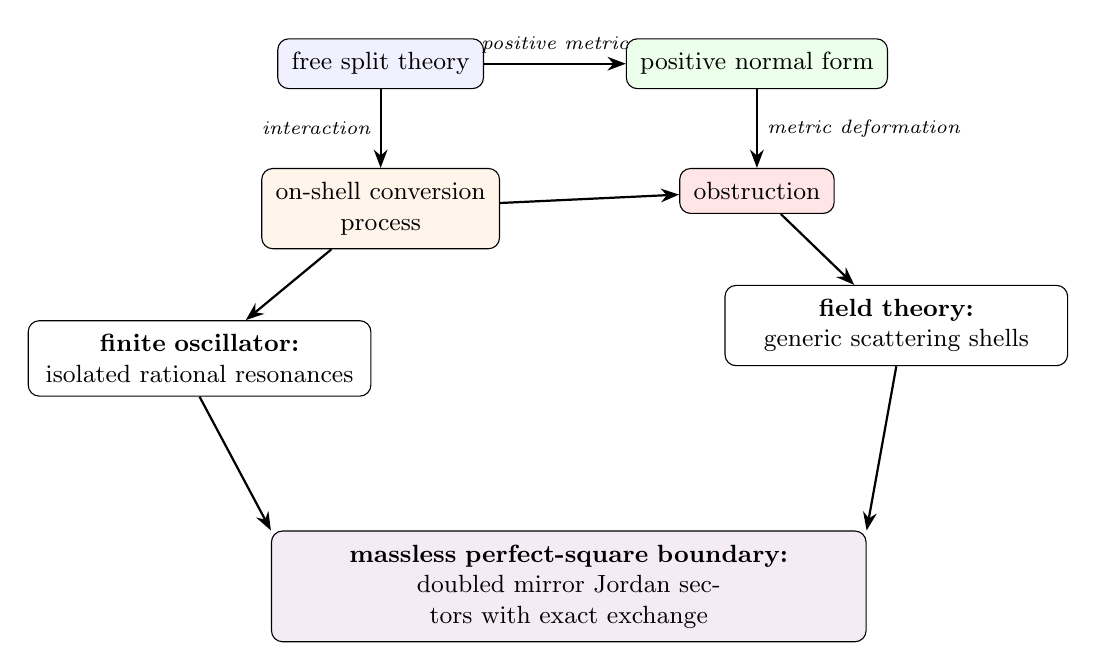
\begin{tikzpicture}[
  box/.style={draw, rounded corners, align=center, inner sep=5pt,
              font=\small},
  arr/.style={-{Stealth}, thick},
  lab/.style={font=\scriptsize\itshape}]
\node[box, fill=blue!6] (free) {free split theory};
\node[box, fill=green!8, right=18mm of free] (pos)
  {positive normal form};
\node[box, fill=orange!8, below=10mm of free] (conv)
  {on-shell conversion\\ process};
\node[box, fill=red!10, below=10mm of pos] (obst)
  {obstruction};
\node[box, below left=9mm and -14mm of conv, text width=40mm]
  (osc) {\textbf{finite oscillator:}\\ isolated rational resonances};
\node[box, below right=9mm and -14mm of obst, text width=40mm]
  (fld) {\textbf{field theory:}\\ generic scattering shells};
\node[box, fill=violet!8, below=42mm of $(conv)!0.5!(obst)$,
      text width=72mm]
  (dbl) {\textbf{massless perfect-square boundary:}\\
         doubled mirror Jordan sectors with exact exchange};
\draw[arr] (free) -- (pos) node[midway, above, lab]{positive metric};
\draw[arr] (free) -- (conv) node[midway, left, lab]{interaction};
\draw[arr] (pos) -- (obst) node[midway, right, lab]{metric deformation};
\draw[arr] (conv) -- (obst);
\draw[arr] (conv) -- (osc);
\draw[arr] (obst) -- (fld);
\draw[arr] (osc.south) -- (dbl.north west);
\draw[arr] (fld.south) -- (dbl.north east);
\end{tikzpicture}
\caption{The interaction mechanism of \cite{paperV}: metric deformation
meets on-shell conversion; isolated resonances in the oscillator become
generic scattering shells in the field theory; at the massless boundary
a doubled exchange structure survives.}
\label{fig:interactions}
\end{figure}

\subsection{Deforming the positive metric}

Perturb the free theory, $H_\zeta=H_0+\zeta V$, and recall the free
Dyson map with $\rho_0H_0\rho_0^{-1}=h_0=h_0^{\dg}$.  One seeks a
corrected map
\begin{equation}
\rho_\zeta=e^{-\frac12(\zeta R_1+\zeta^2R_2+\cdots)}\rho_0,
\end{equation}
keeping the transformed Hamiltonian Hermitian order by order.  At first
order,
\begin{equation}
[h_0,R_1]=v^{\dg}-v,
\qquad v=\rho_0V\rho_0^{-1}.
\end{equation}
The interaction introduces a new ``bad'' non-Hermitian part, and the
correction $R_1$ asks whether the measuring geometry can be adjusted to
absorb it.  The key principle is simple: a correction can remove terms
that move states between \emph{different} energies; it cannot remove a
term that acts entirely among states with exactly the \emph{same}
energy.  When two states have different energies, the metric can
distinguish them; when they have exactly equal energy, the interaction
is resonant and cannot be rotated away.  Technically, the obstruction is
the energy-conserving part of the source,
\begin{equation}
\mathfrak o_+=\Pi_{\ker\operatorname{ad}_{h_0}}S ,
\end{equation}
the projection onto processes satisfying exact free-energy
conservation.

\subsection{A finite oscillator fails only at special resonances}

For the cubic PU interaction at generic unequal frequencies, the
positive metric can be corrected through the computed orders --- the
explicit generators exist and the transformed Hamiltonian is Hermitian.
But at
\begin{equation}
\w_1=3\w_2,
\end{equation}
one high-frequency quantum can convert into three low-frequency quanta
without changing the total energy, and the second-order correction is
obstructed by exactly that conversion operator,
$a_1a_2^{\dg3}-a_1^{\dg}a_2^3$.  At $2\w_1=3\w_2$ a third-order
obstruction appears.  Imagine two musical notes: usually they are
unrelated, but if one note has exactly three times the frequency of the
other, one vibration can split into three without changing the total
energy --- at that point the interaction is perfectly synchronized with
the system.

The $3{:}1$ obstruction is more than a failure of one formula.
Sufficiently excited resonant multiplets develop complex-conjugate
energies, $E_\pm=E_R\pm i\Gamma$, at second order --- certified exactly
in \cite{paperV}.  Where the complex pair persists, no positive-definite
invariant metric can make the Hamiltonian equivalent to an ordinary
self-adjoint one.  Two levels of conclusion must not be merged: this
complex-spectrum statement is established in the verified resonant
oscillator setting; the field-theory result below is presently a
perturbative metric obstruction, not yet a demonstrated complex
spectrum.

\subsection{The momentum continuum turns exceptional resonances into
ordinary scattering}

For an oscillator, the frequencies are fixed numbers and exact
resonances require special ratios.  For a field,
$E_a(k)=\sqrt{k^2+m_a^2}$, and momenta vary continuously: one can
satisfy
\begin{equation}
E_H(k_1)+E_L(k_2)=E_L(k_3)+E_L(k_4)
\end{equation}
together with momentum conservation on open sets of scattering data,
for \emph{any} split masses.  The key process is the branch-changing
scattering $H+L\to L+L$.  Paper~V shows that the second-order
positive-metric source is nonzero on an open part of this shell: the
continuum turns the oscillator's isolated resonance obstruction into a
generic scattering-shell obstruction.  In a small mechanical system,
resonance requires the machine to be tuned to a special ratio; in a
field, particles can change their momentum, and even if their masses
are not specially tuned, their motion can supply the exact energy
match.

The canonical positive completion therefore remains meaningful locally
and perturbatively away from resonant processes, but it cannot
generally be deformed into a positive pointed-sector metric once
branch-changing scattering becomes exactly energy conserving.  One
qualification is essential: this establishes that \emph{no analytic
deformation of the canonical metric} exists there --- not that no
conceivable positive completion of any kind exists.  For the oscillator
with certified complex energies the stronger conclusion is available;
for the field theory the perturbative statement is what is proved.

\subsection{Why the obstruction waits until second order}

The perfect-square cubic vertex is exactly the K\"all\'en polynomial,
$\mathcal V_3=\tfrac12\lambda_{\mathrm K}(p_1^2,p_2^2,p_3^2)$
(Section~\ref{sec:hadamard} notation).  It vanishes for three ordinary
massless legs and has a second-order zero at the confluent massless
point; and the transported reality factors eliminate the first-order
positive obstruction on the physically open decay channel.  So the
positive metric survives the first test.  But at second order, two
cubic interactions combine into a branch-changing $2\to2$ process, and
the obstruction appears: a single interaction event is too constrained
to cause the problem, while two interaction events in sequence can
convert the particles while preserving total energy --- and that is
where the positive geometry fails.

\subsection{A different structure survives: two mirror Jordan sectors}

The perfect-square theory admits an exact rewriting.  Introducing an
auxiliary field and the nonlinear change of variables
$U=e^{\lambda\phi}$, $V=(\psi/\lambda)e^{-\lambda\phi}$,
\begin{equation}
\mathcal L=-\partial_\mu U\,\partial^\mu V
+\frac{\lambda^2}{2}U^2V^2 .
\end{equation}
The constant zero-potential stationary backgrounds form two branches,
$(U_0,0)$ and $(0,V_0)$, and the exact exchange $U\leftrightarrow V$
maps one branch to the other.  Around $(1,0)$ the linearized equations
are $\Box v=0$, $\Box u=\lambda^2v$ --- a Jordan chain generated by the
interaction itself; around $(0,1)$ the chain has the opposite
orientation.  The complete theory thus has two mirror valleys: choosing
one valley gives one orientation of the Jordan system, and the exact
symmetry does not rearrange particles inside that valley --- it carries
the entire valley to its mirror.

Three distinctions matter here.  The exact symmetry belongs globally to
the \emph{extended} $(U,V)$ theory; its expression in the original
$(\phi,\psi)$ variables is a chart-transition map, singular at the
chosen perturbative vacuum; and it is not a ghost-number sign inside
one Fock sector.  It may ultimately form part of an antiunitary
CPT-like structure, but what is proved is a linear sector exchange, not
a quantum CPT theorem.

Finally, the ordinary split-theory ghost parity becomes singular at the
merge.  In the confluent Jordan basis $c=(b_++b_-)/2$,
$d=(b_+-b_-)/\delta$, the branch parity becomes
\begin{equation}
P_\delta=
\begin{pmatrix}0&2/\delta\\ \delta/2&0\end{pmatrix},
\qquad P_\delta^2=1,
\end{equation}
with no bounded limit on a single Jordan chain: as the two particle
types merge, the old rule ``one is even and one is odd'' becomes
infinitely badly conditioned.  The only finite remnant is to exchange
the entire Jordan system with its mirror copy: after doubling by the
oppositely oriented sector, the singular parity becomes a finite sector
exchange --- the linearization of the exact $U\leftrightarrow V$
symmetry around the two mirror backgrounds.

\paragraph{Terminology.}
\emph{Positive pseudo-Hermitian metric}: a positive inner product
obtained by changing the adjoint through a Dyson map.
\emph{Metric deformation}: an order-by-order correction of that inner
product after an interaction is introduced.
\emph{Obstruction}: the energy-conserving part of the unwanted
non-Hermitian interaction that cannot be generated by a metric
correction.
\emph{Pointed sector}: a quantum construction built around one selected
vacuum background.
\emph{Doubled theory}: a completion containing both mirror Jordan
sectors.
\emph{Sector-exchange involution}: the exact map exchanging the two
mirror backgrounds and reversing the Jordan-chain orientation.
\emph{Spectral breaking}: the appearance of complex-conjugate energy
levels, which excludes a positive invariant metric where the complex
spectrum persists.  ``Ghost parity'' is used only with a qualifier:
split branch-number parity, the exact $U\leftrightarrow V$ exchange, or
a (future) antiunitary CPT-like operation are different objects.

\section{Why gravity is not merely five copies of the oscillator}
\label{sec:gravity}

The scalar PU oscillator has no gauge symmetry.  Gravity does.

Consider linearized scalar-free Einstein--Weyl gravity around flat
spacetime: the Einstein term plus a tuned quadratic-curvature term
($\alpha R_{\mu\nu}^2+\beta R^2$ with $\alpha=-3\beta$).  The linearized
spectrum contains a massless graviton with two helicities and a massive
spin-$2$ branch with five helicities \cite{Stelle}.  A naive
polarization-by-polarization treatment might suggest that every massive
helicity belongs to an independent PU pair.  Gauge reduction shows
otherwise \cite{paperIV}: the reduced phase space has the structure
\begin{equation}
\Gamma_{\mathrm{phys}}
\cong
2\,\Gamma_{\mathrm{PU}}\ \oplus\ 2\,\Gamma_-\ \oplus\ \Gamma_- .
\end{equation}
The two helicity-$2$ sectors are genuine fourth-order PU pairs: each
contains a massless graviton mode and a massive ghost partner.  The
helicity-$1$ and helicity-$0$ sectors contain only \emph{unpaired}
second-order massive ghosts: their apparent massless partners lie
entirely in the diffeomorphism gauge orbit and disappear under
reduction.
\keybox{Gauge reduction preserves PU pairing only in helicity $\pm2$.}
This is the first major way in which gravity differs from the scalar
model.

\section{Lorentz covariance forbids hybrid solutions}\label{sec:lorentz}

The five massive helicities $+2,+1,0,-1,-2$ form one irreducible massive
spin-$2$ representation.  They are not five independent species that can
be quantized separately: a Lorentz transformation can mix them.

By Schur's lemma, an invariant Hermitian form on the irreducible
spin-$2$ polarization space is proportional to the identity.  Its sign or
reality assignment must therefore be uniform across all five helicities.
This rules out a tempting hybrid construction in which the helicity-$2$
modes receive the positive PU metric while the helicity-$1$ and
helicity-$0$ ghosts are treated in a Krein space: such an assignment is
not Lorentz covariant.

The gravity paper \cite{paperIV} therefore finds exactly two covariant
completion classes:
\begin{enumerate}
\item a positive pseudo-Hermitian completion in which the full massive
spin-$2$ multiplet has uniformly rotated reality;
\item a Krein completion in which the gravitational field retains
standard reality and the entire massive spin-$2$ multiplet carries a
uniform negative sign relative to the positive massless graviton sector.
\end{enumerate}
The two completions induce the same complex gauge-invariant covariance,
while differing in their involution and completion.  This is the
gravitational version of the real-form distinction of
Figure~\ref{fig:threelevels}.

\section{The conformal Jordan boundary}\label{sec:conformal}

Let the coefficient of the Einstein term tend to zero while the
quadratic-curvature coupling remains fixed.  The massive spin-$2$ mass
then tends to zero, and the different helicity sectors behave
differently \cite{paperIV}.

\paragraph{Helicity $\pm2$.}
The massless and massive branches merge, producing two $\Box^2$ Jordan
systems.  Each polarization contributes two configuration-space
solutions, giving four modes in total.

\paragraph{Helicity $\pm1$.}
The vector ghosts have an ordinary massless limit.  They remain
second-order modes rather than becoming Jordan partners.

\paragraph{Helicity $0$.}
The scalar kinetic normalization tends to zero.  At the conformal point a
new Weyl gauge symmetry appears,
$\delta h_{\mu\nu}=2\sigma\eta_{\mu\nu}$: the scalar direction becomes
null in the presymplectic form and is removed by the quotient.

The conformal count is therefore $4+2+0=6$.  The positive
split-frequency metric runs to infinite Cartan distance and has no
nondegenerate positive continuation through the Jordan boundary; the
complex spectral covariance and the standard-reality Krein form can
continue, provided the newly null Weyl direction is quotiented out.  The
algebra of observables changes rank at the boundary, so convergence must
be formulated on a fixed regular family of observables --- most naturally
through gauge- and Weyl-invariant curvature quantities.  (Boundary
constructions that instead \emph{remove} one branch of the solution
space, as in \cite{Maldacena}, and the richer phase diagram at nonzero
cosmological constant \cite{LuPope,DeserWaldron}, are related but
distinct stories.)

\paragraph{What Paper V predicts for interacting gravity.}
The interaction results of Section~\ref{sec:interactions} have not yet
been carried out for gravity, but they supply the machinery and the
expected shape.  The massive spin-$2$ multiplet can participate in
branch-changing processes such as $h+h\leftrightarrow M$,
$h+M\leftrightarrow h+h$, and $M+M\leftrightarrow h+M$, depending on
kinematics and the cubic vertices.  The natural test is: construct the
free positive real form of the massive spin-$2$ sector; transport the
cubic Einstein--Weyl vertices; project their anti-Hermitian parts onto
energy-conserving scattering shells; test whether the positive metric
deformation is obstructed; and search for any doubled or CPT-compatible
completion.  Interacting gravity has \emph{not} been shown to fail;
what Paper~V supplies is the obstruction machinery, and it makes
branch-changing gravitational scattering the natural next calculation.

\section{What was already solved, and what is new}\label{sec:new}

It is important not to claim that earlier work failed to solve anything.
Bender and Mannheim solved the free unequal-frequency oscillator's
spectral and positive-norm problem by introducing a nontrivial metric
\cite{BM2008PRL,BM2008PRD}.  Bateman and Turok supplied a controlled
Krein-space treatment of the massless resonant scalar theory, including a
ghost-parity interpretation \cite{BT2026}.  The new contribution is a
classification and unification (Figure~\ref{fig:dependency}):

\begin{description}
\item[Paper I \cite{paperI}] reconstructs the Bender--Mannheim generator
from the symplectic normal-form data and classifies the diagonalizers and
the algebraic metric freedom.
\item[Paper II \cite{paperII}] proves that the canonical Bender--Mannheim
transformation is the minimum-Cartan-distortion representative, embeds
the result in a general orthogonal projection principle, and separates
the physical Dyson equivalence from the auxiliary identity-embedding
obstruction.
\item[Paper III \cite{paperIII}] separates metric geometry, vacuum
covariance, dynamical Jordan structure, and field representation theory;
identifies the common spectral divided-difference covariance, its
confluent limit, and its fourth-order Hadamard structure.
\item[Paper IV \cite{paperIV}] determines how gauge reduction and Lorentz
covariance change the classification in gravity: the helicity
stratification, the exclusion of covariant hybrid completions, and the
conformal Jordan boundary.
\item[Paper V \cite{paperV}] tests which free completions survive
interactions: the deformation and obstruction theory of
Section~\ref{sec:interactions} --- generic deformability, resonance
obstructions, spectral complexification, the generic continuum shell
obstruction, and the exact doubled sector-exchange symmetry.
\end{description}

In one paragraph: the five papers develop a progression from free
classification to interacting obstruction theory.  The first two derive
and geometrically characterize the canonical positive Pais--Uhlenbeck
metric.  The third separates this metric from the universal complex
vacuum covariance and follows the theory to its Jordan boundary.  The
fourth determines how gauge reduction and Lorentz covariance modify the
classification in quadratic gravity.  The fifth asks whether the free
completions survive interactions: the positive metric deforms away from
resonances but is obstructed by exactly energy-conserving
branch-changing processes --- on isolated rational loci in the
oscillator and on generic scattering shells in the field theory ---
while at the massless perfect-square boundary an exact doubled exchange
survives between two oppositely oriented Jordan sectors.  The resulting
question is no longer simply whether a ghost can be assigned positive
norm, but which real form and completion remain compatible with the
actual interactions of the theory.

\begin{figure}[t]
\centering
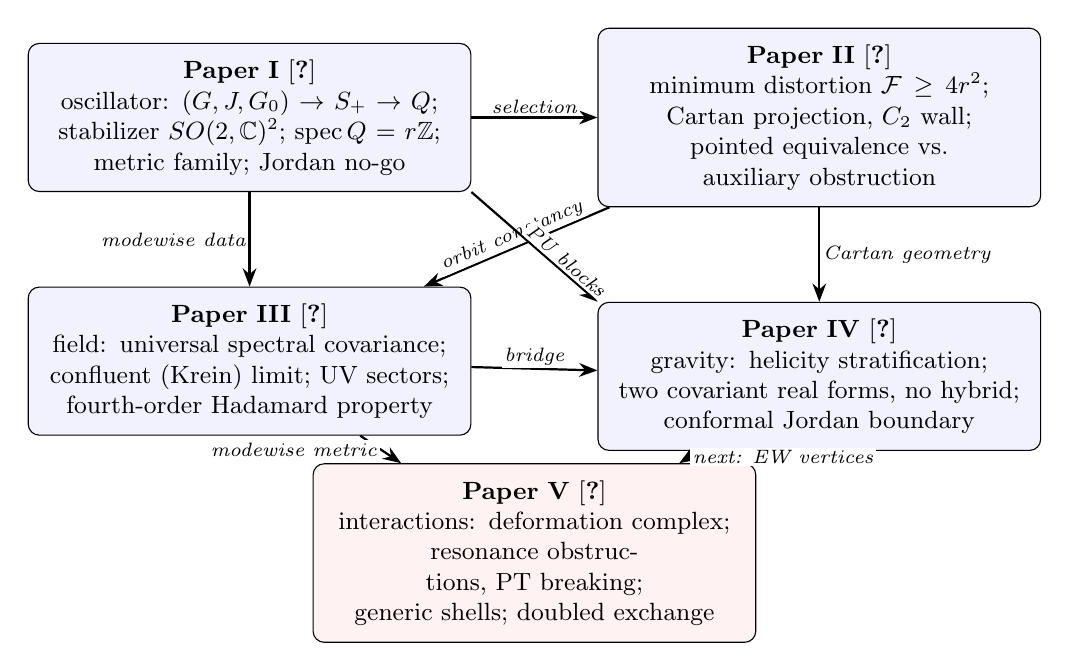
\begin{tikzpicture}[
  pap/.style={draw, rounded corners, align=center, inner sep=6pt,
              font=\small, fill=blue!5, text width=52mm},
  arr/.style={-{Stealth}, thick},
  lab/.style={font=\scriptsize\itshape, midway, fill=white, inner sep=1pt}]
\node[pap] (p1)
  {\textbf{Paper I} \cite{paperI}\\
   oscillator: $(G,J,G_0)\to S_+\to Q$;\\
   stabilizer $SO(2,\C)^2$; spec\,$Q=r\Z$;\\
   metric family; Jordan no-go};
\node[pap, right=16mm of p1] (p2)
  {\textbf{Paper II} \cite{paperII}\\
   minimum distortion $\mathcal F\ge4r^2$;\\
   Cartan projection, $C_2$ wall;\\
   pointed equivalence vs.\\ auxiliary obstruction};
\node[pap, below=12mm of p1] (p3)
  {\textbf{Paper III} \cite{paperIII}\\
   field: universal spectral covariance;\\
   confluent (Krein) limit; UV sectors;\\
   fourth-order Hadamard property};
\node[pap, below=12mm of p2] (p4)
  {\textbf{Paper IV} \cite{paperIV}\\
   gravity: helicity stratification;\\
   two covariant real forms, no hybrid;\\
   conformal Jordan boundary};
\draw[arr] (p1) -- (p2) node[lab, above]{selection};
\draw[arr] (p1) -- (p3) node[lab, left]{modewise data};
\draw[arr] (p2) -- (p3) node[lab, above, sloped]{orbit constancy};
\draw[arr] (p3) -- (p4) node[lab, above]{bridge};
\draw[arr] (p2) -- (p4) node[lab, right]{Cartan geometry};
\draw[arr] (p1.south east) -- (p4.north west)
  node[lab, sloped, above, pos=0.7]{PU blocks};
\node[pap, fill=red!5, below=12mm of $(p3)!0.5!(p4)$] (p5)
  {\textbf{Paper V} \cite{paperV}\\
   interactions: deformation complex;\\
   resonance obstructions, PT breaking;\\
   generic shells; doubled exchange};
\draw[arr] (p3) -- (p5) node[lab, left]{modewise metric};
\draw[arr] (p4) -- (p5) node[lab, right]{next: EW vertices};
\end{tikzpicture}
\caption{Dependency structure of the five technical papers.}
\label{fig:dependency}
\end{figure}

The combined novelty is therefore not a new claim that one particular
ghost Hamiltonian can be rewritten positively.  It is the statement that:
\keybox{The known positive and Krein constructions are different
real-form completions of a common complex spectral structure.  Their
admissibility and continuation are controlled by symplectic geometry,
Cartan projection, gauge reduction, Lorentz representation theory, and
Jordan degeneration.}

\section{What remains open}\label{sec:open}

The first interaction-level answers are now in
(Section~\ref{sec:interactions}), but they sharpen rather than exhaust
the open questions.

For the positive completion: the deformation exists away from
resonances, but does any nonanalytic or differently pointed positive
completion evade the shell obstruction?  Does the field theory, like
the oscillator, develop complex energies (complex finite-volume levels
or non-real resonance poles)?  Does renormalization preserve the metric
structure?  (See \cite{QQG2024} for a recent PT-based proposal at the
interacting level.)

For the doubled structure: can the exact sector exchange be implemented
as an operator on a quantum completion?  Are the two pointed sectors
superselected in infinite volume, or do parity vacua
$(|0_A\rangle\pm|0_B\rangle)/\sqrt2$ exist?  Can a probability
interpretation be built on the doubled space, and is the exchange part
of an antiunitary CPT-like operation?

For gravity: do the cubic Einstein--Weyl vertices obstruct the positive
real form of the massive spin-$2$ sector through branch-changing
scattering, as Paper~V's machinery predicts is testable?  Does the
real-form classification survive on curved backgrounds and at nonzero
cosmological constant \cite{LuPope,DeserWaldron}?

These are no longer vague versions of ``does the ghost go away?''  They
are concrete algebraic and analytic tests.

\section{Conclusion}\label{sec:conclusion}

The traditional ghost problem combines several logically separate issues:
classical stability, spectral boundedness, norm positivity, field
reality, vacuum covariance, representation theory, gauge reduction, and
Jordan degeneration.

The results now form a five-level hierarchy:
\keybox{1. The free complex spectral theory can be identified.\\
2. Its positive and Krein real forms can be classified.\\
3. The canonical positive metric is geometrically selected.\\
4. Interactions test the deformability of these real forms.\\
5. On-shell conversion processes generate genuine obstructions.}
The PU oscillator shows that a Hamiltonian that appears ghostlike in one
real form may possess a positive pseudo-Hermitian completion in another;
the minimum-distortion theorem explains why the Bender--Mannheim metric
is geometrically canonical; the free field theory shows that the metric
may become singular while the complex vacuum covariance remains regular;
and gravity adds gauge symmetry and Lorentz covariance, which remove
some pairings and force the massive spin-$2$ multiplet to be treated as
a whole.

The interaction results complete the picture: the positive
pseudo-Hermitian construction is a valid local resolution of the free
and nonresonant weakly interacting theory.  It is not generically
stable under exactly energy-conserving branch-changing processes.  In
field theory, the momentum continuum makes such processes far more
common than in a finite oscillator.  At the massless perfect-square
boundary, the surviving structure is instead an exact exchange between
two oppositely oriented Jordan sectors.

The resulting view is neither that higher-derivative ghosts are
automatically harmless nor that they automatically invalidate a theory.
The refined question is:
\keybox{Not ``Can the ghost be removed?''\ but ``Which completion
survives the allowed interactions?''}
Once the ingredients --- complex dynamics, real form, involution,
observable algebra, completion, and now interaction stability --- are
separated, the existing positive and indefinite constructions cease to
look like unrelated tricks.  They become different parts of one
geometric, representation-theoretic, and deformation-theoretic
framework.

\paragraph{Verification.}
Every finite-dimensional, variational, symplectic, and modewise
distributional identity quoted in this introduction is machine-verified
in the repository accompanying the series
\cite{paperI,paperII,paperIII,paperIV,paperV} (symbolic SymPy audits,
high-precision numerical regression, and a Lean~4 formalization of the
paper-I core with zero unproved placeholders); the technical papers state
precisely which of their conclusions are analytic rather than
machine-checked.

\begin{thebibliography}{99}

\bibitem{Ostrogradsky}
M.~Ostrogradsky,
\emph{M\'emoire sur les \'equations diff\'erentielles relatives au
probl\`eme des isop\'erim\`etres},
M\'em.\ Acad.\ St.\ P\'etersbourg \textbf{VI 4} (1850) 385.

\bibitem{Woodard}
R.~P.~Woodard,
\emph{The theorem of Ostrogradsky},
arXiv:1506.02210.

\bibitem{PU1950}
A.~Pais and G.~E.~Uhlenbeck,
\emph{On field theories with non-localized action},
Phys.\ Rev.\ \textbf{79} (1950) 145.

\bibitem{BenderBoettcher}
C.~M.~Bender and S.~Boettcher,
\emph{Real spectra in non-Hermitian Hamiltonians having PT symmetry},
Phys.\ Rev.\ Lett.\ \textbf{80} (1998) 5243.

\bibitem{BM2008PRL}
C.~M.~Bender and P.~D.~Mannheim,
\emph{No-ghost theorem for the fourth-order derivative Pais--Uhlenbeck
oscillator model},
Phys.\ Rev.\ Lett.\ \textbf{100} (2008) 110402.

\bibitem{BM2008PRD}
C.~M.~Bender and P.~D.~Mannheim,
\emph{Exactly solvable PT-symmetric Hamiltonian having no Hermitian
counterpart},
Phys.\ Rev.\ D \textbf{78} (2008) 025022, arXiv:0804.4190.

\bibitem{BT2026}
S.~Bateman and N.~Turok,
\emph{Escape from Ostrogradsky via hidden ghost parity},
arXiv:2607.00096.

\bibitem{SGH1992}
F.~G.~Scholtz, H.~B.~Geyer and F.~J.~W.~Hahne,
\emph{Quasi-Hermitian operators in quantum mechanics and the variational
principle},
Ann.\ Phys.\ \textbf{213} (1992) 74.

\bibitem{Mostafazadeh2010}
A.~Mostafazadeh,
\emph{Pseudo-Hermitian representation of quantum mechanics},
Int.\ J.\ Geom.\ Meth.\ Mod.\ Phys.\ \textbf{7} (2010) 1191.

\bibitem{Mannheim2021}
P.~D.~Mannheim,
\emph{Solution to the ghost problem in higher-derivative gravity},
arXiv:2109.12743.

\bibitem{Stelle}
K.~S.~Stelle,
\emph{Classical gravity with higher derivatives},
Gen.\ Rel.\ Grav.\ \textbf{9} (1978) 353;
Phys.\ Rev.\ D \textbf{16} (1977) 953.

\bibitem{paperI}
\emph{Canonical positive symplectic diagonalization of the
Pais--Uhlenbeck oscillator}, companion paper (Paper~I) and verification
repository, 2026.

\bibitem{paperII}
\emph{The Pais--Uhlenbeck metric as a minimum-distortion principle, and
the representation problem for the fourth-order field}, companion paper
(Paper~II), 2026.

\bibitem{paperIII}
\emph{The universal vacuum of the fourth-order scalar field: metric
orbits, Fock sectors, and the Krein boundary}, companion paper
(Paper~III), 2026.

\bibitem{paperIV}
\emph{Gauge reduction and the completion problem in fourth-order gravity:
PU pairing, covariant real forms, and the conformal Jordan boundary},
companion paper (Paper~IV), 2026.

\bibitem{paperV}
\emph{Interaction obstructions, resonant PT breaking, and doubled Jordan
symmetry in fourth-order theories}, companion paper (Paper~V), 2026.

\bibitem{Folland}
G.~B.~Folland,
\emph{Harmonic Analysis in Phase Space},
Princeton University Press, 1989.

\bibitem{Bhatia2007}
R.~Bhatia,
\emph{Positive Definite Matrices},
Princeton University Press, 2007.

\bibitem{Mostow1955}
G.~D.~Mostow,
\emph{Self-adjoint groups},
Ann.\ of Math.\ \textbf{62} (1955) 44.

\bibitem{KempfNess1979}
G.~Kempf and L.~Ness,
\emph{The length of vectors in representation spaces},
in: Algebraic Geometry, Lecture Notes in Math.\ \textbf{732}, Springer,
1979, 233.

\bibitem{GLR2005}
I.~Gohberg, P.~Lancaster and L.~Rodman,
\emph{Indefinite Linear Algebra and Applications},
Birkh\"auser, 2005.

\bibitem{Kato}
T.~Kato,
\emph{Perturbation Theory for Linear Operators},
Springer, 1966.

\bibitem{Heiss2012}
W.~D.~Heiss,
\emph{The physics of exceptional points},
J.\ Phys.\ A \textbf{45} (2012) 444016.

\bibitem{vN1939}
J.~von Neumann,
\emph{On infinite direct products},
Compos.\ Math.\ \textbf{6} (1939) 1.

\bibitem{Radzikowski}
M.~J.~Radzikowski,
\emph{Micro-local approach to the Hadamard condition in quantum field
theory on curved space-time},
Commun.\ Math.\ Phys.\ \textbf{179} (1996) 529.

\bibitem{BrunettiFredenhagen}
R.~Brunetti and K.~Fredenhagen,
\emph{Microlocal analysis and interacting quantum field theories},
Commun.\ Math.\ Phys.\ \textbf{208} (2000) 623.

\bibitem{HollandsWald}
S.~Hollands and R.~M.~Wald,
\emph{Local Wick polynomials and time ordered products of quantum fields
in curved spacetime},
Commun.\ Math.\ Phys.\ \textbf{223} (2001) 289.

\bibitem{Maldacena}
J.~Maldacena,
\emph{Einstein gravity from conformal gravity},
arXiv:1105.5632.

\bibitem{LuPope}
H.~L\"u and C.~N.~Pope,
\emph{Critical gravity in four dimensions},
Phys.\ Rev.\ Lett.\ \textbf{106} (2011) 181302, arXiv:1101.1971.

\bibitem{DeserWaldron}
S.~Deser, E.~Joung and A.~Waldron,
\emph{Partial masslessness and conformal gravity},
J.\ Phys.\ A \textbf{46} (2013) 214019, arXiv:1208.1307.

\bibitem{QQG2024}
J.~Kubo and J.~Kuntz,
\emph{Unitarity through PT symmetry in quantum quadratic gravity},
arXiv:2410.08278.

\end{thebibliography}

\end{document}
